%%%%%%%%%%%%%%%%%%%%%%%%%%%%%%%%%%%%%%%%%
% Cv BENGO
% LuaLaTeX Template
% Version 1.12.0 (11/04/2024)
%
% Original authors:
% Ged Lex (gedlex@hotmail.ch)
%
% Important note:
% This template must be compiled with LuaLaTeX, the below lines will ensure this
%!TEX TS-program = lualatex
%!TEX encoding = UTF-8 Unicode
%%%%%%%%%%%%%%%%%%%%%%%%%%%%%%%%%%%%%%%%%

%----------------------------------------------------------------------------------------
%	PACKAGES AND OTHER DOCUMENT CONFIGURATIONS

%----------------------------------------------------------------------------------------
\documentclass[rightPos]{ReCeiVe}      % By default, use 'letterpaper' for US letter
%\geometry{letterpaper, % paper size
%          left=1.75cm, right=1.75cm, top=1.5cm, bottom=1.5cm, footskip=.6cm, headsep=.5cm, % margins
%          showframe}                  % show geometry frame
%          heightrounded}              % avoid underfull vbox warning
 \usepackage{xcolor} 
 \usepackage{multicol}
% Color for highlights
%\definecolor{highlight}{HTML}{FF0000} % Specify your own color
%\colorlet{highlight}{white}           % Set predefined color
% Default colors include: darkgray, gray, lightgray, lightblue, orange, red, concrete

%Colors for text - uncomment and modify
%\definecolor{darktext}{HTML}{FF0000}
%\definecolor{text}{HTML}{FF0000}
%\definecolor{graytext}{HTML}{FF0000}
%\definecolor{lighttext}{HTML}{414141}

%----------------------------------------------------------------------------------------
%	PERSONAL INFORMATION
%	Comment any of the lines below if they are not required
%----------------------------------------------------------------------------------------
\background{pics/background5.pdf}
\photo[rectangle,edge,nofill,left]{5cm}{pics/pp2.pdf}
\name{Dylane}{Bengono}
\homepage{bio.link/chaneldy}
\mobile{237 6 91 45 77 03}
\email{chaneldylanebengono@gmail.com}
\linkedin{chanel-dylane-b-91b850194/}
\github{Bengo237}
\extrainfo{24 years old}

%\twitter{@twit}
%\xing{xing name}
%\stackoverflow{SOid}{SOname}
%\skype{skypeid}
%\reddit{reddit account}
%\extrainfo{info}

\position{Security Engineer | DevSecOps} % Your expertise/domains
\headwords{Engineer, software enthusiast, technical enthusiast and carpenter} % Some keywords to describe you

\quote{"Some people see things as they are and ask why. I dream of things that never were and ask why not." - Robert Kennedy}

%----------------------------------------------------------------------------------------
%	SIDEBAR CONTENT
%	Fill in the information you would like to add to your sidebar
%----------------------------------------------------------------------------------------

\aboutMe {Dedicated Cybersecurity Analyst,proficient in safeguarding endpoints, providing DevOps support, deploying SIEM solutions, and implementing NAC frameworks. Actively participates in Capture The Flag competitions for continuous skill enhancement and innovative problem-solving}
\skillset[label/0\hfill +500 h]{ Pentest/.8,IT Standards and References/.7, Network Security/.9, Virtualization and Cloud/.8, Cryptography/.6 , IAM/.6}
\languages{{English/C1}, {French/C2}}


% Usage: \userSection[<section title>]{<content>}
% \userSection[title]{content}

%----------------------------------------------------------------------------------------
\begin{document}
% Print the header
% Usage: \makecvheader[<position>]
\makecvheader
% Print the sidebar
% Usage: \makecvsidebar[xOffset/value,yOffset/value,noRadius|radius]
\makecvsidebar
%----------------------------------------------------------------------------------------
%	CV/RESUME CONTENT
%	Each section is imported separately, open each file in order to modify it
%----------------------------------------------------------------------------------------
\vspace{3mm}
\section{Professional Experience}

\cventry
{Security Engineer} % Job title
{adorsys GmbH \& Co. KG} % Organization
{Remote, CM} % Location
{Dec/2023 - Present} % Date
\begin{cvitems}
\item {Technical implementation of client endpoint protection (EPP) solutions.}
\item {Provided DevOps support for EUDI Wallet, ensuring seamless integration and deployment.}
\item {Acted as a Project Maintainer, overseeing the development lifecycle and ensuring project objectives were met.}
\end{cvitems}

\cventry
{Cybersecurity Engineer Intern} % Job title
{Port Authority of Kribi, PAK} % Organization
{Kribi, CM} % Location
{02/2023 - 08/2023} % Date
{
\begin{cvitems}
\item {Designed and implemented a Security Information and Event Management (SIEM) system to enhance threat detection capabilities.}
\item {Performed testing and deployment of computer hardware to optimize network security infrastructure.}
\item {Provided user assistance and support, ensuring smooth operations and addressing security concerns promptly.}
\end{cvitems}
}

\cventry
{Pre-Engineer Network Security Intern} % Job title
{General Delegation for National Security, DGSN} % Organization
{Yaoundé, CM} % Location
{07/2022 - 10/2022} % Date
{
\begin{cvitems}
\item {Designed and implemented a Network Access Control (NAC) system to regulate network access and enhance security posture.}
\item {Conducted asset mapping exercises to identify critical network assets and vulnerabilities.}
\item {Implemented risk management strategies and performed network monitoring to mitigate potential threats.}
\end{cvitems}
}

\cventry
{IT Manager} % Job title
{Association APSF and ACMALEF} % Organization
{Yaoundé, CM} % Location
{08/2022 - present} % Date
{
\begin{cvitems}
\item {Administered the website amouretpartage.ovh, ensuring its smooth operation and security.}
\item {Managed various social media pages, effectively communicating with stakeholders and promoting organizational objectives.}
\end{cvitems}
}
\section{Education}
\cventry
{Master of Engineering, Cybersecurity and Digital Investigation} % Degree
{National Advanced School of Engineering of Yaounde} % Institution
{Yaoundé, CM} % Location
{09/2018 - 08/2023} % Date
\begin{multicols}{2}

\begin{itemize}
  \item Linux Administration and Shell
  \item Azure
  \item Kubernetes
  \item Containerization with Docker
  \item Office 365
  \item IT Support
  \item Python
  \item Bash scripting
\end{itemize}
\begin{itemize}
  \item Hashing Algorithms: MD4, MD5, SHA
  \item Asymmetric Encryption: RSA 
  \item Symmetric Encryption: Triple DES, RC4, AES
  \item Secure Communication Protocols: IPsec, SSL/TLS, SSH
  \item Oauth Protocol
\end{itemize}

\subsection*{IAM (Identity and Access Management)}
\begin{itemize}
  \item PacketFence NAC, Cisco Cnac 
  \item Zabbix | Nagios
  \item WaZUH, Splunk, IBM Qradar
  \item Keycloak
\end{itemize}

\subsection*{Standards, References and Regulations}
\begin{itemize}
  \item ANSSI Hygiene Guide, PSSI, SMSI, PCA
  \item ISO 27001, 27002, 27005
  \item GDPR
\end{itemize}

\subsection*{Pentest}
\begin{itemize}
  \item Kali Linux, Metasploit, Nmap, Nessus
\end{itemize}

\subsection*{Networks}
\begin{itemize}
  \item DNS, DHCP, NAT
  \item Security Equipment: Firewall, Netbox
  \item MPLS, OSI, SNMP, TCP/IP
\end{itemize}

\subsection*{Virtualization and Cloud}
\begin{itemize}
  \item Cloud computing (IaaS, PaaS, SaaS)
  \item VMware ESXi, Xen
\end{itemize}

\end{multicols}
\section{Awards and Honors}
\begin{cvhonors}

\cvhonor
{Finalist} % Position
{Innovation Challenge Kamany Talent Academy (KTA SARL)} % Event
{Yaoundé, Cameroon} % Location
{2020} % Date
\cvhonor
{9th/39} % Position
{Cybersecurity Experts Olympiad 2021, AEC-CTF} % Event
{Online} % Location
{2021} % Date

\end{cvhonors}


\section{Certifications}

\begin{center}
{\color{blue} \rule{\linewidth}{1mm}}
\end{center}

\renewcommand{\figurename}{} % Supprimer le libellé "Figure"

\begin{figure}[htbp]
    \centering
    \begin{minipage}[t]{0.45\textwidth}
        \centering
        \href{https://aspen.eccouncil.org/VerifyBadge?type=certification&a=k0oDOJ1A+oFRUFqxi7ayyh4IMBf2VEh1mGt6WtgWbL4=}{
        
\includegraphics[height=2cm]{badge/CSCU.png}}
        \caption*{Certified Secure Computer User}
    \end{minipage}
    \hfill
    \begin{minipage}[t]{0.45\textwidth}
        \centering
        \href{https://www.coursera.org/account/accomplishments/certificate/VH72LKQENH77}{
        \includegraphics[height=2cm]{badge/CCT.png}}
        \caption*{Certified Cyber Security Technician}
    \end{minipage}
\end{figure}

\begin{figure}[htbp]
    \centering
    \begin{minipage}[t]{0.45\textwidth}
        \centering
        \href{https://www.credly.com/badges/1367a47a-2cf3-408d-a7be-26adaaf1066d}{
        \includegraphics[height=2cm]{badge/PENT.png}}
        \caption*{Penetration Tester}
    \end{minipage}
    \hfill
    \begin{minipage}[t]{0.45\textwidth}
        \centering
        \href{https://www.credly.com/badges/bc5666c7-c769-46c7-9ebd-d31458ad103d/linked_in_profile}{
        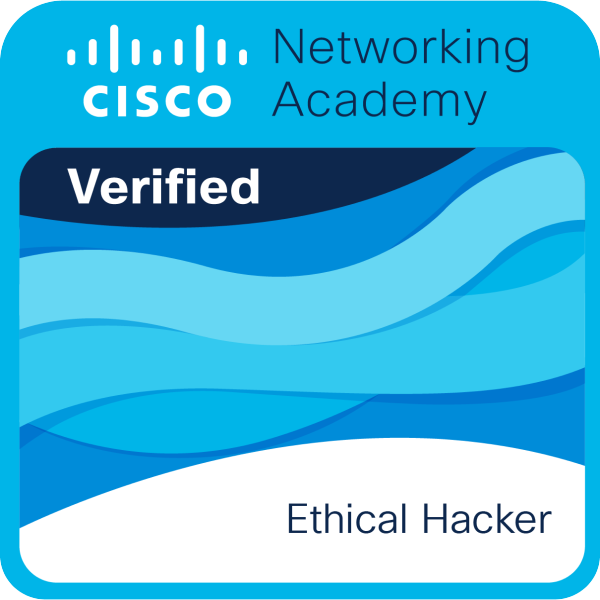
\includegraphics[height=2cm]{badge/ceh cisco.png}}
        \caption*{Cisco Ethical Hacker}
    \end{minipage}
\end{figure}

\begin{figure}[htbp]
    \centering
    \begin{minipage}[t]{0.45\textwidth}
        \centering
        \href{https://app.kajabi.com/certificates/0cb8dd89}{
        \includegraphics[height=2cm]{badge/CPTA-v2.png}}
        \caption*{Certified Purple Team Analyst}
    \end{minipage}
    \hfill
    \begin{minipage}[t]{0.45\textwidth}
        \centering
        \href{https://drive.google.com/file/d/16sqn1fYpKX8QDNoTrmbRuvluLTrWHJgE/view?usp=sharing}{
        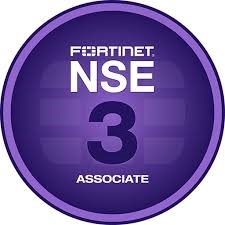
\includegraphics[height=2cm]{badge/nse.png}}
        \caption*{Network Security Associate}
    \end{minipage}
\end{figure}







\vspace{3mm}
%\section{Awards and Honors}
\begin{cvhonors}

\cvhonor
{Finalist} % Position
{Innovation Challenge Kamany Talent Academy (KTA SARL)} % Event
{Yaoundé, Cameroon} % Location
{2020} % Date
\cvhonor
{9th/39} % Position
{Cybersecurity Experts Olympiad 2021, AEC-CTF} % Event
{Online} % Location
{2021} % Date

\end{cvhonors}


\section{Certifications}

\begin{center}
{\color{blue} \rule{\linewidth}{1mm}}
\end{center}

\renewcommand{\figurename}{} % Supprimer le libellé "Figure"

\begin{figure}[htbp]
    \centering
    \begin{minipage}[t]{0.45\textwidth}
        \centering
        \href{https://aspen.eccouncil.org/VerifyBadge?type=certification&a=k0oDOJ1A+oFRUFqxi7ayyh4IMBf2VEh1mGt6WtgWbL4=}{
        
\includegraphics[height=2cm]{badge/CSCU.png}}
        \caption*{Certified Secure Computer User}
    \end{minipage}
    \hfill
    \begin{minipage}[t]{0.45\textwidth}
        \centering
        \href{https://www.coursera.org/account/accomplishments/certificate/VH72LKQENH77}{
        \includegraphics[height=2cm]{badge/CCT.png}}
        \caption*{Certified Cyber Security Technician}
    \end{minipage}
\end{figure}

\begin{figure}[htbp]
    \centering
    \begin{minipage}[t]{0.45\textwidth}
        \centering
        \href{https://www.credly.com/badges/1367a47a-2cf3-408d-a7be-26adaaf1066d}{
        \includegraphics[height=2cm]{badge/PENT.png}}
        \caption*{Penetration Tester}
    \end{minipage}
    \hfill
    \begin{minipage}[t]{0.45\textwidth}
        \centering
        \href{https://www.credly.com/badges/bc5666c7-c769-46c7-9ebd-d31458ad103d/linked_in_profile}{
        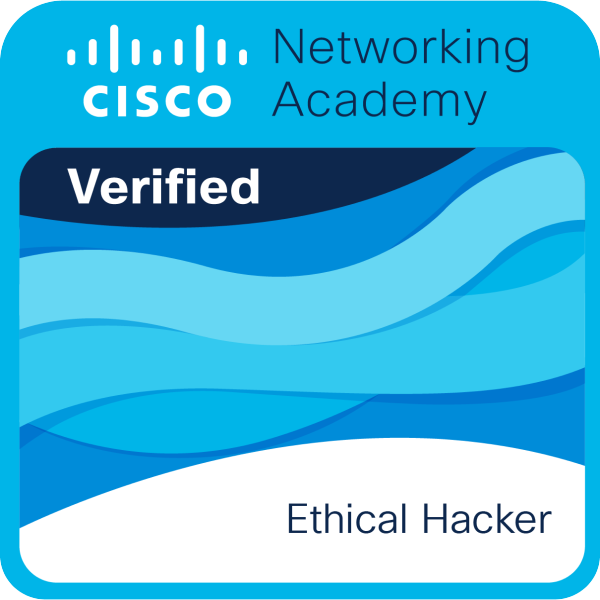
\includegraphics[height=2cm]{badge/ceh cisco.png}}
        \caption*{Cisco Ethical Hacker}
    \end{minipage}
\end{figure}

\begin{figure}[htbp]
    \centering
    \begin{minipage}[t]{0.45\textwidth}
        \centering
        \href{https://app.kajabi.com/certificates/0cb8dd89}{
        \includegraphics[height=2cm]{badge/CPTA-v2.png}}
        \caption*{Certified Purple Team Analyst}
    \end{minipage}
    \hfill
    \begin{minipage}[t]{0.45\textwidth}
        \centering
        \href{https://drive.google.com/file/d/16sqn1fYpKX8QDNoTrmbRuvluLTrWHJgE/view?usp=sharing}{
        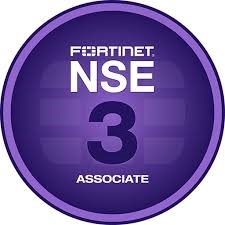
\includegraphics[height=2cm]{badge/nse.png}}
        \caption*{Network Security Associate}
    \end{minipage}
\end{figure}









%----------------------------------------------------------------------------------------
\end{document}
